\graphicspath{{./fig_Exec/}}
%

\section{CBCの実行}

次のようなディレクトリ構成を仮定し,3Dcavityの例題を実行します.
標準のMakefileでコンパイルすると,コンパイル済みのsphere実行モジュールはbinディレクトリに格納されます.
パラメータファイルは,cavity.xmlとします.

{\small
\begin{program}
Examples
  |
  +- 3Dcavity
  |    +-cavity.xml
  :
\end{program}
}

カレントディレクトリをexamples/3Dcavityとし,sphereの実行モジュールのディレクトリにパスを通しておくと,以下のように実行できます.

{\small
\begin{program}
$ sphere cavity.xml
\end{program}
}

%
\pagebreak
\section{出力ファイル}

\subsection{出力ファイルの種類と指定}
\label{sec:log_files}

CBCソルバークラスを実行すると,\textbf{表\ref{tbl:logfiles}}に示すファイルが生成されます.
これらのファイル名\index{ふぁいる@ファイル!りれき@履歴---}は\hyperlink{tgt:output_data}{OutputData}で指定します.
また,logファイルについては,\hyperlink{tgt:log}{Log}セクションで生成の有無を指定します.

\begin{table}[htdp]
\caption{実行時にできるファイル}
\begin{center}
\small
\begin{tabular}{lll}\toprule
カテゴリ & attrタグ指定 & 出力内容\\ \midrule
解析条件情報 & condition & 計算条件,前処理,ソルバー起動時のログ\\
領域情報 & - & 並列計算時の計算領域の分割に関する情報\\ 
性能情報 & profiling & 実行時間サンプリング出力ファイル\\ \hline
基本履歴 & log\_base & ステップ数,時刻,反復回数,収束状況などの情報\\
コンポーネント履歴 & log\_compo & 内部境界のモニタ情報\\
流量収支履歴 & log\_domainflux & 計算外部領域における流入出流量,平均速度の情報\\
反復履歴 & log\_iteration & 反復解法の収束履歴\\ 
サンプリング履歴 & log\_sampling & サンプリング指定時の出力ファイル\\ 
壁面情報履歴 & log\_wall\_info & 壁面に関する情報の履歴\\ \hline
瞬時値データ & Velocity & 速度の瞬時値\\
& Pressure & 圧力の瞬時値\\
& Temperature & 温度の瞬時値\\
平均値データ & AvrVelocity & 速度の時間平均値\\
& AvrPressure & 圧力の時間平均値\\
& AvrTemperature & 温度の時間平均値\\
派生データ & tp & 全圧\\
& vrt & 渦度\\
& helicity & ヘリシティ\\
& i2vgt & 速度勾配テンソルの第2不変量\\ 
\bottomrule
\end{tabular}
\end{center}
\label{tbl:logfiles}
\end{table}

\textbf{表\ref{tbl:logfiles}}の履歴と瞬時値・平均値のデータ出力については,出力インターバルを指定できます.
出力インターバルは\hyperlink{tgt:interval}{Interval}セクションに記述し,各項目独立に,ステップと時刻のどちらによっても指定可能です.

%
\pagebreak
\subsection{解析条件情報 [condition.txt]}
\label{sec:condition.txt}
ソルバーを実行すると,condition.txtファイル\index{ふぁいる@ファイル!condition---}が生成されます.
このファイルはCBCソルバークラス起動時のログで,ボクセルファイルを読み込み,ソルバーに必要な境界条件の設定に係わる前処理,チェック内容などが\textbf{表\ref{tbl:log-section}}に示す各セクション毎に記録されています.

\begin{table}[htdp]
\caption{condition.txtファイルの表示項目}
\begin{center}
\small
\begin{tabular}{ll}\toprule
セクション名 & 表示内容\\ \midrule
Domain Information & 計算領域の寸法,配列サイズ,格子ピッチ,原点座標\\
Voxel file information & 計算するボクセルファイルの名称や含まれる情報\\
Memory required for Preprocesor & 前処理に必要なメモリ要求量(概算)\\
XML Table Info. & Model\_Settingタグに記述された内容\\
XML Components & コンポーネントの種類と個数\\
Voxel Model Info. & voxelファイルに含まれるIDの情報\\
Medium List & Model\_Settingタグに記述された媒質情報\\
Component List & 各コンポーネントのID,要素数,媒質など\\
Component Information & 各コンポーネントの詳細な情報\\
Memory required for Solver & ソルバー本体で必要なメモリ要求量(概算)\\
Solver Control Parameters & 制御パラメータ\\
Simulation Parameters & 物理量のパラメータ\\
Initial Values for Physical Variables & 初期値の情報\\
Effective cells and Open Area of Computational Domain& 計算対象セル数と各外部境界面における開口面積の割合\\
Outer Boundary Conditions & 外部境界条件\\ 
Monitor Information & XML指定によるモニター情報\\ \bottomrule
\end{tabular}
\end{center}
\label{tbl:log-section}
\end{table}

%
\pagebreak
\subsection{領域情報 [DomainInfo.txt]}
領域全体の情報,および領域分割された各サブドメインの配列サイズ,領域サイズ,原点座標の情報が表示されます.
また,各領域に含まれる境界条件コンポーネントのBoundingBoxのインデクス情報が含まれます.

\begin{indentation}{2zw}{0zw}
{\small 
\begin{program}
>> Global Domain Information

imax, jmax, kmax    =            73            28            28

(dx, dy, dz) [m] / [-] = ( 2.0000e-02 2.0000e-02 2.0000e-02) / ( 3.5714e-02 3.5714e-02 3.5714e-02)
(ox, oy, oz) [m] / [-] = ( 2.0000e-02 2.0000e-02 2.0000e-02) / ( 3.5714e-02 3.5714e-02 3.5714e-02)
(Lx, Ly, Lz) [m] / [-] = ( 1.4600e+00 5.6000e-01 5.6000e-01) / ( 2.6071e+00 1.0000e+00 1.0000e+00)

Domain    0
ix, jx,  kx        [-] =             37            28            28
(ox, oy, oz) [m] / [-] = ( 2.0000e-02 2.0000e-02 2.0000e-02) / ( 3.5714e-02 3.5714e-02 3.5714e-02)
(Lx, Ly, Lz) [m] / [-] = ( 7.4000e-01 5.6000e-01 5.6000e-01) / ( 1.3214e+00 1.0000e+00 1.0000e+00)
no            Label    ID    i_st    i_ed    j_st    j_ed    k_st    k_ed
 1              Air     4       0       0       0       0       0       0

Domain    1
ix, jx,  kx        [-] =             36            28            28
(ox, oy, oz) [m] / [-] = ( 7.6000e-01 2.0000e-02 2.0000e-02) / ( 1.3571e+00 3.5714e-02 3.5714e-02)
(Lx, Ly, Lz) [m] / [-] = ( 7.1999e-01 5.6000e-01 5.6000e-01) / ( 1.2857e+00 1.0000e+00 1.0000e+00)
no            Label    ID    i_st    i_ed    j_st    j_ed    k_st    k_ed
 1              Air     4      14      17       1      28       1      28
\end{program}
}
\end{indentation} 

%
\pagebreak
\subsection{基本履歴 [history\_base.log]}
\label{sec:baseinfo}

標準履歴ファイル\index{ふぁいる@ファイル!ひょうじゅんりれき@標準履歴---}は,下記のような履歴情報\index{りれき@履歴}が出力されます.
この履歴情報は選択された時間積分スキームや反復解法の収束判定ノルムの種類などにより出力項目は異なります.
下記の計算例では,時間積分にEuler陽解法を用いた流動解析を行い,圧力Poisson方程式の反復解の収束判定のノルムに速度の発散の最大値を用いています.
各欄のラベルの説明を\textbf{表\ref{tbl:out_label}}に示します.

標準出力とhistory\_base.logファイルには同じ内容が出力され,時刻と速度の次元は有次元となっています.収束判定のノルムの種類については,\textbf{表\ref{tbl:norm-type}}を参照のこと.ノルムの次元は慣例的に無次元としています.\\

\begin{indentation}{2zw}{0zw}
{\small 
\begin{program}
    step      time[sec]  v_max[m/s]   ItrP   V_div_Max     deltaP       avrP     deltaV       avrV
       1   4.000000e-05  0.0000e+00      1  2.3687e-07  1.476e-14 -7.991e-17  5.493e-15  5.493e-15
       2   8.000001e-05  6.8344e-13      1  1.1870e-06  2.602e-09  1.069e-10  1.878e-10  1.878e-10
       3   1.200000e-04  2.4322e-08      1  2.8058e-06  9.901e-09  5.841e-10  8.173e-10  1.003e-09
       4   1.600000e-04  1.1977e-07      1  4.6971e-06  2.073e-08  1.737e-09  1.942e-09  2.937e-09
       5   2.000000e-04  3.2279e-07      1  6.7086e-06  3.395e-08  3.859e-09  3.487e-09  6.404e-09
       6   2.400000e-04  6.6904e-07      1  8.8056e-06  4.920e-08  7.234e-09  5.350e-09  1.171e-08
       7   2.800000e-04  1.1826e-06      1  1.0970e-05  6.639e-08  1.214e-08  7.459e-09  1.910e-08
\end{program}
}

\begin{table}[htdp]
\caption{履歴ファイルの出力項目}
\begin{center}
\small
\begin{tabular}{ll} \toprule
Label & 説明\\ \midrule
step & 計算ステップ数\\
time & 時刻\\
v\_max & 速度の最大値\\
ItrP & 圧力ポアソンの反復回数\\
V\_div\_Max & 反復の収束判定に用いるノルムの種類とその値.上記の場合は速度の発散値の最大値を用いています.\\
& 指定するノルムの種類により,ヘッダの記述が変わります.\\
deltaP & 圧力の1ステップの変化量の自乗和平方根 $\sqrt{ \sum_{i,j,k}^{Max} {\|\delta{p}\|}_{2} }$\\
avrP   & 圧力の平均値\\
deltaV & 速度の1ステップの変化量の自乗和平方根 $\sqrt{ \sum_{i,j,k}^{Max} {\|\delta{v}\|}_{2} }$\\
avrV   & 速度の平均値\\
deltaT & 温度の1ステップの変化量の自乗和平方根 $\sqrt{ \sum_{i,j,k}^{Max} {\|\delta{\theta}\|}_{2} }$\\ 
avrT   & 温度の平均値\\ \bottomrule
\end{tabular}
\end{center}
\label{tbl:out_label}
\end{table}


下記には,熱流動計算を流動計算にEuler陽解法,温度場は対流項にEuler陽解法,拡散項にEuler陰解法を用いた履歴の出力例を示す.ItrTは温度の反復解法の反復回数を示し,続くT\_Res\_L2\_Rはノルムに相対残差を選択していることを示します.また,dTは温度の1ステップの変化量のRMSです.

{\small
\begin{program}
step       time       v_max  ItrP P_res_L2_R ItrT T_res_L2_R        dP        dV        dT
   1 1.2500e-04  0.0000e+00     1 0.0000e+00    6 9.5454e-05 0.000e+00 0.000e+00 2.654e-01 
   2 2.5000e-04  0.0000e+00   201 5.2254e-05   11 2.1408e-05 3.962e+05 1.338e+02 2.583e-01 
   3 3.7500e-04  1.0464e+01   201 4.3515e-05    9 8.5652e-05 3.901e+05 2.599e+02 2.495e-01 
   4 5.0000e-04  3.0324e+01   201 3.5191e-05    9 2.8809e-05 3.839e+05 3.750e+02 2.386e-01 
   5 6.2500e-04  5.7543e+01   201 2.8940e-05    8 6.5638e-05 3.789e+05 4.750e+02 2.269e-01 
   6 7.5000e-04  9.2345e+01   201 2.5224e-05    8 3.7452e-05 3.769e+05 5.584e+02 2.164e-01 
   7 8.7500e-04  1.3304e+02   201 2.3655e-05    8 2.4891e-05 3.797e+05 6.287e+02 2.091e-01
\end{program}
}

\end{indentation}

%
\hypertarget{tgt:history_compo}{\subsection{コンポーネント履歴 [history\_compo.log]}}

コンポーネントに関連する履歴\index{ふぁいる@ファイル!こんぽーねんとりれき@コンポーネント履歴---}を出力します.

\begin{indentation}{2zw}{0zw}
{\small 
\begin{program}
    step         time      V[011]     Va[050]    DPa[050]   MonV[020]   MonP[020]  MonTP[020]
       1   2.9605e-03 -1.6511e-02  0.0000e+00  0.0000e+00  0.0000e+00  1.0132e+05  0.0000e+00
       2   5.9211e-03 -6.6040e-02  0.0000e+00  0.0000e+00  0.0000e+00  1.0132e+05  0.0000e+00
       3   8.8816e-03 -1.4857e-01  0.0000e+00  0.0000e+00  0.0000e+00  1.0132e+05  0.0000e+00
       4   1.1842e-02 -2.6406e-01  0.0000e+00  0.0000e+00  0.0000e+00  1.0132e+05  0.0000e+00
       5   1.4803e-02 -4.1247e-01  0.0000e+00  0.0000e+00  0.0000e+00  1.0132e+05  0.0000e+00
       6   1.7763e-02 -5.9375e-01  0.0000e+00  0.0000e+00  0.0000e+00  1.0132e+05  0.0000e+00
       7   2.0724e-02 -8.0783e-01  0.0000e+00  0.0000e+00  0.0000e+00  1.0132e+05 -2.8205e-33
       8   2.3684e-02 -1.0546e+00  0.0000e+00  0.0000e+00 -7.5572e-24  1.0132e+05 -7.6584e-19
       9   2.6645e-02 -1.3340e+00  0.0000e+00  0.0000e+00 -6.7933e-17  1.0132e+05 -1.3883e-11
      10   2.9605e-02 -1.6460e+00  0.0000e+00  0.0000e+00 -2.4990e-13  1.0132e+05 -7.4992e-08
\end{program}
}

上記の例では,ID=11に速度を指定し,その平均速度を出力しています.ID=50には熱交換器を割り当て,平均通過流速と圧力損失量を表示しています.また,ID=20はモニタで,平均速度,圧力,全圧を出力しています.各表示量は有次元値で,\textbf{表\ref{tbl:monitor-display}}に示す項目が表示されます.

\begin{table}[htdp]
\caption{コンポーネント履歴ファイルの出力項目}
\begin{center}
\small
\begin{tabular}{lll} \toprule
カテゴリー & コンポーネント & 表示項目\\ \midrule
Vec\_Face & &\\
& Dirichlet & 平均速度 $V\,[m/s]$\\
& & 温度指定の場合,流入熱量 $Q\,[W]$\\
Forcing\_Volume & &\\
& HEX & 熱交換機平均通過流量 $Va\,[m^3/s]$\\
& & 平均圧力損失量 $DPa [Pa]$\\
& DARCY & 平均通過風速の速度成分 $U,\,V,\,W,\,[m/s]$\\
Heat\_Face & &\\
& Direct & 熱流束 $q\,[W/m^2]$\\
& Heat\_Transfer\_N & 熱流束 $q\,[W/m^2]$\\
& Heat\_Transfer\_S & 熱流束 $q\,[W/m^2]$\\
& Heat\_Transfer\_B & 熱流束 $q\,[W/m^2]$\\
& Iso\_Thermal & 熱流束 $q\,[W/m^2]$\\
& Radiation & 熱流束 $q\,[W/m^2]$\\
Heat\_Volume & &\\
& Heat\_Src &\\
& Cnst\_Temp &\\
Monitor & &\\
& Velocity & 平均速度 $MonV\,[m/s]$\\
& Pressure & 平均圧力 $MonP\,[Pa]$\\
& Temperature & 平均温度 $MonT\,[K\,or\,C]$\\
& TotalPressure & 平均全圧 $MonTP\,[Pa]$\\
\bottomrule
\end{tabular}
\end{center}
\label{tbl:monitor-display}
\end{table}

\end{indentation}

%
\pagebreak
\subsection{流量収支履歴 [history\_domainflux.log]}
計算領域の外部境界における流量と速度の履歴\index{ふぁいる@ファイル!りゅうりょうりれき@流量履歴---}を出力します.
Qは断面流量$[m^3/s]$を,Balanceは計算内部領域への流入出する流量の和を示します.
Vは有効断面平均速度$[m/s]$を表すが,BCで述べるように流出断面を指定している場合には指定される対流速度モードの値となります.

\begin{indentation}{2zw}{0zw}
{\small
\begin{program}
    step         time         Q:X-   ...      Q:Z+ >>      Balance         V:X-   ...   V:Z+
     756 1.890020e+00  -7.5980e-02     -1.3623e-01 >>   6.5136e-01  -1.3155e-03  -8.6816e-04
     757 1.892520e+00  -7.6318e-02     -1.3660e-01 >>   6.5357e-01  -1.3214e-03  -8.7049e-04
     758 1.895020e+00  -7.6656e-02     -1.3696e-01 >>   6.5578e-01  -1.3273e-03  -8.7283e-04
\end{program}
}
\end{indentation}

%
\pagebreak
\subsection{反復履歴 [history\_iteration.log]}
Poissonの反復履歴\index{ふぁいる@ファイル!はんぷくりれき@反復履歴---}を示します.
ノルムの選択に速度の発散を指定している場合には,計算領域内の位置が出力されます.

\begin{indentation}{2zw}{0zw}
{\small 
\begin{program}
step=               1  time= 6.666667e-03  Itration          Norm (     i,      j,      k)
                                                  1  3.765856e-05 (     5,     46,     92)
step=               2  time= 1.333333e-02  Itration          Norm (     i,      j,      k)
                                                  1  1.076603e-04 (     5,     46,     92)
step=               3  time= 2.000000e-02  Itration          Norm (     i,      j,      k)
                                                  1  1.823895e-04 (     5,     46,     92)
step=               4  time= 2.666667e-02  Itration          Norm (     i,      j,      k)
                                                  1  2.715028e-04 (     5,     46,     92)
step=               5  time= 3.333334e-02  Itration          Norm (     i,      j,      k)
                                                  1  3.676064e-04 (     5,     46,     92)
\end{program}
}
\end{indentation}


%
\pagebreak
\subsection{サンプリング履歴 [history\_sampling.log]}
\label{sec:XML_sampling_history}
XMLの座標値指定によるサンプリング結果を出力します.
第\ref{chpt:monitor}章をご覧ください.


%
\pagebreak
\hypertarget{tgt:profile}{\subsection{性能情報}}
実行時のタイミングを測定し,サマリーを表示します.各項目の表示内容を\textbf{表\ref{tbl:timing_label}}に示します.

\begin{indentation}{2zw}{0zw}
{\small 
\begin{program}
----------------------------------------------------------------
Report of Timing Statistics
Total execution time            = 5.960922e+00 [sec]
Total time of measured sections = 5.461881e+00 [sec]

Statistics per MPI process [Node Average]
Lavel       |call |             accumulated time            |       flop | messages[Bytes]
            |     |   avr[sec]  avr[%]   sdv[s] avr/call[s] |   avr         sdv         speed
------------------+------------+----------------------------+-------------------------------------
Search Vmax :  25   6.0695e-02   1.11  0.000e+00  2.4278e-03   4.325e+08  0.000e+00    6.64 Gflops
assign BC   :  75   2.1376e-03   0.04  0.000e+00  2.8502e-05   0.000e+00  0.000e+00    0.00 Mflops
Copy Array  :  50   3.1872e-01   5.84  0.000e+00  6.3744e-03   0.000e+00  0.000e+00    0.00 Mflops
Pseudo Vec  :  25   3.0864e+00  56.51  0.000e+00  1.2345e-01   2.180e+10  0.000e+00    6.58 Gflops
P Vec FluxBC:  25   1.3652e-02   0.25  0.000e+00  5.4609e-04   1.055e+07  0.000e+00  737.20 Mflops
Pvec. EE    :  25   1.3234e-01   2.42  0.000e+00  5.2938e-03   2.595e+08  0.000e+00    1.83 Gflops
Pvec. BC    :  25   2.2888e-03   0.04  0.000e+00  9.1552e-05   3.870e+04  0.000e+00   16.12 Mflops
PvecFace BC :  25   8.4519e-04   0.02  0.000e+00  3.3807e-05   1.325e+04  0.000e+00   14.95 Mflops
assign Array:  50   3.9125e-02   0.72  0.000e+00  7.8251e-04   0.000e+00  0.000e+00    0.00 Mflops
Div CC      :  25   2.7460e-01   5.03  0.000e+00  1.0984e-02   8.939e+08  0.000e+00    3.03 Gflops
Poi Src. BC :  25   9.2988e-03   0.17  0.000e+00  3.7195e-04   5.499e+06  0.000e+00  563.93 Mflops
Poi Setup   :  25   1.5258e-05   0.00  0.000e+00  6.1035e-07   0.000e+00  0.000e+00    0.00 Mflops
Poi SOR2SMA :  50   1.7074e-01   3.13  0.000e+00  3.4149e-03   7.370e+10  0.000e+00  401.97 Gflops
Poi BC      :  50   9.1314e-05   0.00  0.000e+00  1.8262e-06   0.000e+00  0.000e+00    0.00 Mflops
Prj Vec CF  :  25   5.7449e-01  10.52  0.000e+00  2.2979e-02   1.398e+09  0.000e+00    2.27 Gflops
Prj Vec CFBC:  25   1.0159e-02   0.19  0.000e+00  4.0636e-04   1.930e+04  0.000e+00    1.81 Mflops
Prj Vec CC  :  25   3.0391e-01   5.56  0.000e+00  1.2156e-02   1.038e+09  0.000e+00    3.18 Gflops
Vec. BC     :  25   4.4822e-05   0.00  0.000e+00  1.7929e-06   0.000e+00  0.000e+00    0.00 Mflops
Div CF      :  25   1.0764e-01   1.97  0.000e+00  4.3057e-03   2.019e+08  0.000e+00    1.75 Gflops
P Norm Dmax :  25   4.0273e-02   0.74  0.000e+00  1.6109e-03   8.651e+07  0.000e+00    2.00 Gflops
Updt Vec.   :  25   7.0383e-03   0.13  0.000e+00  2.8153e-04   0.000e+00  0.000e+00    0.00 Mflops
Oflow Vel   :  25   2.9467e-02   0.54  0.000e+00  1.1786e-03   1.455e+07  0.000e+00  471.01 Mflops
Avr Space   :  25   2.7546e-01   5.04  0.000e+00  1.1018e-02   6.632e+08  0.000e+00    2.24 Gflops
H Stdout    :  25   1.0623e-03   0.02  0.000e+00  4.2495e-05   0.000e+00  0.000e+00    0.00 Mflops
H Base      :  25   7.7629e-04   0.01  0.000e+00  3.1051e-05   0.000e+00  0.000e+00    0.00 Mflops
H DomainFlux:  25   3.5381e-04   0.01  0.000e+00  1.4152e-05   0.000e+00  0.000e+00    0.00 Mflops
Monitoring  :  25   1.3113e-05   0.00  0.000e+00  5.2452e-07   0.000e+00  0.000e+00    0.00 Mflops
H Component :  25   2.0313e-04   0.00  0.000e+00  8.1253e-06   0.000e+00  0.000e+00    0.00 Mflops
------------------+------------+----------------------------+-------------------------------------
Total       |                5.461881e+00                      1.005e+11              17.14 Gflops
\end{program}
}

\begin{table}[htdp]
\caption{タイミングレポートの表示内容}
\begin{center}
\small
\begin{tabular}{ll}\toprule
項目 & 内容\\ \midrule
Initialize              & 初期化部分\\
Pseudo Vector           & 疑似速度ベクトルの計算部分\\
BC for u* and u         & 疑似速度と速度に対する境界条件\\
Projection to $u^{n+1}$ & 速度の射影\\
Judge convergence       & 同時緩和の収束判定,$\nabla (u_i)$の計算を含む\\
LES                     & LES部分\\
Src of Poisson          & Poisson方程式のソース項\\
Simultaneous Relaxation & 同時緩和の反復部分\\
Poisson LS (only)       & Poissonの線形計算のみ\\
BC for Pressure         & 圧力の境界条件\\
Thermal Convection      & 温度計算の対流項部分\\
Thermal BC              & 温度計算の境界条件\\
Thermal Diffusion       & 温度計算の拡散項部分\\
Post                    & 後処理\\ \midrule
call & 実行回数\\
accm & 積算時間 [sec]\\
avr  & 1回あたりの平均実行時間 [sec]\\ \bottomrule

\end{tabular}
\end{center}
\label{tbl:timing_label}
\end{table}

\end{indentation}

%
\pagebreak
\subsection{その他のファイル}
デバッグ時のBCIndex.txtファイルには,コンポーネント\index{コンポーネント}に関する情報が表示されます.

%
\pagebreak
\subsection{ボクセルファイル}
\label{sec:generated_voxel}
組み込み例題の場合には,内部で生成されたボクセルファイル\index{ふぁいる@ファイル!ぼくせる@ボクセル---}がexample.svxなどとして書き出されます.
また,ユーザ問題でMonitor\_Listが指定されている場合には,サンプル点(セルセンター値)のボクセルにID=255が割り当てられたボクセルファイルが出力されます.

%
\pagebreak
\subsection{結果ファイル}

計算結果は,デフォルトでsph\index{ふぁいる@ファイル!sph---}ファイルフォーマット出力で書き出される.これらは,V-Isioで可視化できます.


%
\pagebreak
\subsection{メモリ使用量の情報}
\label{sec:memory_req}
CBCソルバークラスでは,実行中において,必要なときに必要な量だけメモリを使用する方針です.
このため,プリプロセスとメインループ(計算部分実行中)でメモリ使用量は異なります.
プログラム起動中に必要な最大メモリ量をcondition.txt中に表示します.
\textbf{表\ref{tbl:temporary_in}},\textbf{表\ref{tbl:temporary_out}}にそれぞれファイル入出力時のテンポラリのメモリ使用量のパターンを示します.

svxファイルの並列処理時の読み込みは,マスターノードのみでファイルをオープンします.
svxは内部に幾つかのデータレコードを持てるが,各データ毎に読み込み処理を順次行うので,テンポラリとしては全計算領域サイズ$\times$4Byteの大きさとなります.

sbxファイルの並列処理時の読み込みもマスターノードのみでファイルをオープンします.
また,sbxファイルは圧縮機能があり,圧縮時と非圧縮時で使用するテンポラリサイズが異なります.
圧縮時にはブロックサイズ(デフォルトで,ガイドセルを含むIJ面のボクセルサイズ)のテンポラリを用いてデータを展開します.
非圧縮時にはマスターノードで全計算領域サイズのテンポラリ配列にデータを読み込み,送信先ノードのローカルサイズの配列を用意し,これを送信バッファとして用いて送信します.

\begin{table}[htdp]
\caption{入力時にテンポラリに確保するメモリ量}
\begin{center}
\small
\begin{tabular}{llll} \toprule
動作モード    & svx                           & sbx                      & sph\\ \midrule
逐次         & 全計算領域サイズ$\times$4Byte   & 圧縮時,ブロックサイズ      & 全計算領域サイズ\\
             &                              & 非圧縮時,全計算領域サイズ   & \\
並列(非分散) & マスターノードで全計算          & 圧縮時,マスターでブロックサ  & マスターで全領域サイズ \\
             & 領域サイズ$\times$4Byte       & イズ+送信先ノードのローカル  & +送信先ノードのローカルサイズ\\
             &                              & サイズ(4Byte)              & \\
             &                              & 非圧縮時,全計算領域サイズ+  & \\ 
             &                              & 送信先ノードのローカルサイズ  & \\ 
並列(分散)   & 設定なし                      & 設定なし                   & テンポラリ不使用 \\ \bottomrule
\end{tabular}
\end{center}
\label{tbl:temporary_in}
\end{table}

\begin{table}[htdp]
\caption{出力時におけるテンポラリのメモリ使用量}
\begin{center}
\small
\begin{tabular}{llll} \toprule
動作モード   & sph\\ \midrule
逐次        & 全計算領域サイズ\\
並列(非分散)& マスターで全領域サイズ+受信先ノードのローカルサイズサイズ(4Byte)\\
並列(分散)  & テンポラリ不使用 \\ \bottomrule
\end{tabular}
\end{center}
\label{tbl:temporary_out}
\end{table}

%
\pagebreak
\section{並列計算}
\label{sec:parallel_exec}

\subsection{MPI並列}
\label{sec:MPI}
本節では,MPI通信ライブラリを用いたプロセス並列\index{ぷろせすへいれつ@プロセス並列}の実行について説明します.
並列計算\index{へいれつけいさん@並列計算}は,まず\ref{sec:install MPI}で述べたように並列モジュールを指定し,コンパイルします.
実行時には,mpirun\index{mpirun}コマンドでsphereモジュールを起動します.

{\small
\begin{program}
$ mpirun -np 2 sphere hogehoge.xml
\end{program}
}

%
\pagebreak
\subsection{スレッド並列}
\label{sec:thread}
本節では,共有メモリでのスレッド並列\index{すれっどへいれつ@スレッド並列}の実行について説明します.

%
\pagebreak
\subsection{Multiply-Connected Partitioning}
\label{sec:multibox}
管路網などの内部流を効率よく並列計算するためのしくみとして,多重連結領域分割(Multiply-Connected Partitioning, MCP,または通称マルチボックス)による並列計算ができます.
これは\textbf{図\ref{fig:multibox}}に示すような全計算領域を計算量がほぼ同じになるような部分領域に分割し,並列計算を行う方法です.
MCPで計算する場合には,計算ボクセルのフォーマットとしてsbxを指定して出力する必要があります.

\begin{figure}[htbp]
\begin{center}
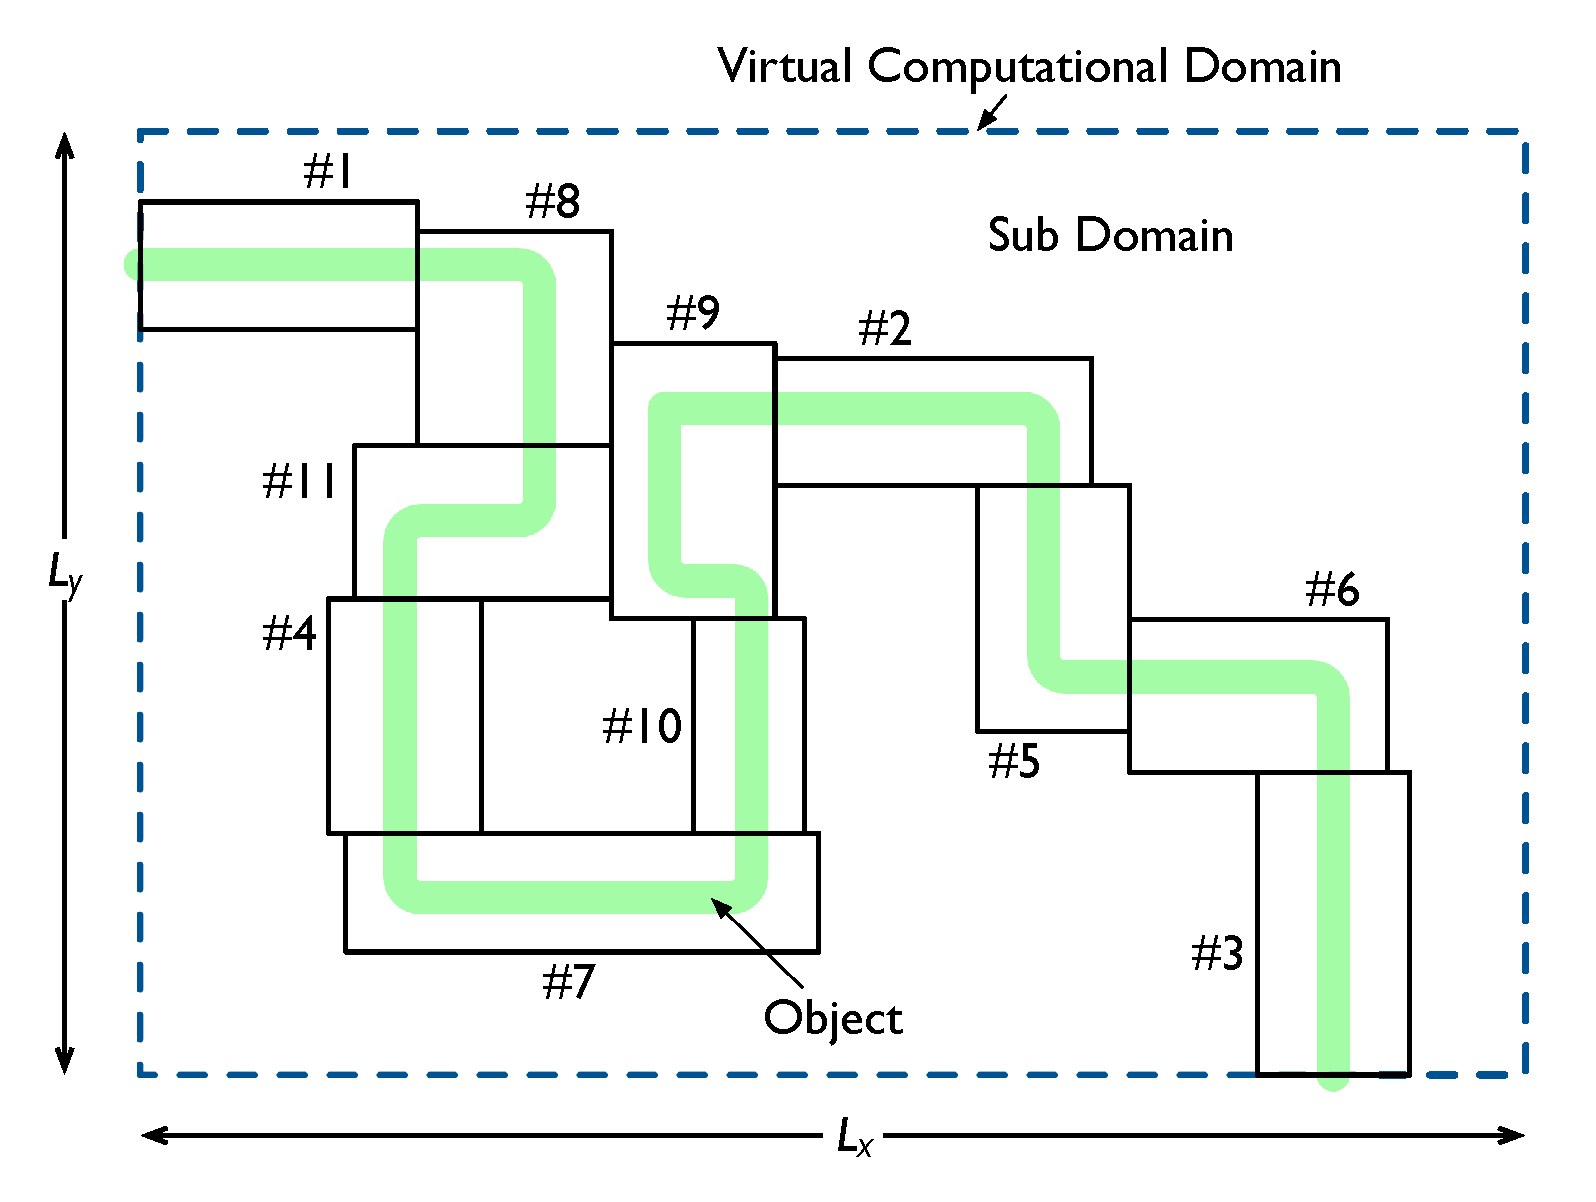
\includegraphics[width=12cm,clip]{mBox.eps}
\end{center}
\caption{Schematic of Multiply-Connected Partitioning}
\label{fig:multibox}
\end{figure}

以下に,マルチボックス計算の手順を示します.
\begin{enumerate}
\item ボクセル生成 V-Xgenを用いてsbxフォーマットのボクセルファイルを作成します.
\item マルチボックスツール sphMbxTool\footnote{09\_Multibox.pdfを参照}を用いて分割ファイルを作成します.
\item XMLファイル 分割ファイル情報をDomainInfoセクションのMBXTBLタグに記述します.


{\small
\begin{program}
<DomainInfo>
  <VoxelSize   ix="64" jx="64" kx="64" />
  <VoxelOrigin ox="0.0" oy="0.0" oz="0.0" />
  <VoxelPitch  dx="0.0" dy="0.0" dz="0.0" />
  <Param name="MDMTBL" dtype="STRING" value="xml/medium.xml" />
  <Param name="BCTBL"  dtype="STRING" value="xml/boundary.xml" />
  <Param name="MBXTBL" dtype="STRING" value="xml/multibox.xml">
</DomainInfo>
\end{program}
}


\item 計算実行 \verb|$mpirun -np 8 sphere hoge.xml|
\end{enumerate}


%
\pagebreak
\section{各プラットホームにおける実行}
\label{sec:exec_platforms}

\subsection{RICC}
\label{sec:exec_RICC}
バッチジョブのスクリプトファイル例を示します.

\begin{indentation}{3zw}{0zw}

{\small
\begin{program}
#!/bin/sh

#----- qsub option
#MJS: -mpc
#MJS: -proc 64
#MJS: -thread 1
#MJS: -mem 1200mb
#MJS: -time 24:00:00
#MJS: -eo
#MJS: -rerun Y
#MJS: -cwd
#MJS: -parallel openmpi

#----- FTLcommand
#FTLDIR: $MJS_CWD
#FTL_SUFFIX: off
#FTL_RANK_FORMAT: 3
#FTL_NO_RANK: off
#
#<BEFORE>
#ALL: sphere_f
#0: P32E_resize_5mm_CutWS.svx
#</BEFORE>
#
#<BEFORE_R>
#ALL: xml
#</BEFORE_R>
#
#<AFTER>
#0: *.sph, *.txt, *.log
#</AFTER>

#----- Program execution
mpirun ./sphere_f xml/p32e.xml
\end{program}
}
\end{indentation}

\pagebreak
次に,利用頻度の高いコマンド類を示します.

\begin{indentation}{3zw}{0zw}
\begin{description}
\item[■] ジョブ投入
{\small
\begin{program}
$ qsub go.sh
\end{program}}

\item[■] ジョブ状態表示
{\small
\begin{program}
$ qstat -m  使用メモリ量
$ qstat -p  プライオリティ
$ qstat -w  実行待ち理由の表示
\end{program}}

\item[■] 実行中Jobの標準出力表示
{\small
\begin{program}
$ qcat REQID
\end{program}}

\item[■] Job優先度変更
{\small
\begin{program}
$ qalter -p <PRIORITY> <REQID>
\end{program}}

\item[■] mpcの計算ノード上のファイル一覧
{\small
OPTIONはlsコマンドと同じである.
\begin{program}
$ qls REQID[@RankID] [OPTION]
\end{program}}

\item[■] mpcの計算ノード上のファイルを取得します.
{\small
\begin{program}
$ qget REQID[@RankID] file
\end{program}}

\end{description}
\end{indentation}

